\section{Kıyaslama düzeneği}\label{sec:setup}

\subsection{Örnekler}
\begin{description}
\item[mTSPLib (16).] eil51, berlin52, eil76, rat99; $k\in\{2,3,5,7\}$, depo
şehir~1'de \citep{necula2015}.
\item[Literatür kümesi (\LitCount).] \citet{hehao2023,hehaoxia2024} tarafından kullanılan
min--maks kıyaslama kümeleri $\mathbb{S}$ ve $\mathbb{L}$'nin TSPLIB tabanlı örnekleri:
kroA200, lin318, rat783, pcb1173 ve nrw1379, fl1400, d1655, u2152, pr2392,
pcb3038, fl3795, fnl4461, rl5915; her biri $k\in\{3,5,10,20\}$ ile, depo
şehir~1'de. Depo ve uzaklık kuralının doğruluğu denetlenmiştir: en uzak şehrin baskın olması nedeniyle
bilinen en iyi çözümünün (BKS) optimal olduğu kanıtlanmış her örnekte
(ör.\ pcb1173, $k=20$: 6528.86), $2\max_v d(\text{city }1,v)$ ifadesi bu değeri
ikinci ondalık basamağa kadar yeniden üretmiştir. Referans değer olarak, yayımlanmış BKS ile
\citet{hehaoxia2024} tarafından elde edilen en iyi sonuçtan daha iyi olanı alınmıştır.
\item[Sentetik bahçeler (\OrchCount).] Tamamlayıcı çalışmamızda \citep{asil2026frame} sunulan yöntemle üretilmiştir:
$(r,c)$ değerleri $(20,25)$, $(40,50)$, $(60,80)$ ve
$(80,125)$ olan $r\times c$ ağaç, sıra aralığı
4\,m, ağaç aralığı 2\,m, \%5 eksik ağaç, $\sigma=0.2$\,m konum gürültüsü,
dikdörtgen ya da L biçimli tarlalar, rastgele yönelim, iki tohum ve
$k\in\{4,8,16\}$; $n$, \OrchNmin{} ile \OrchNmax{} arasında değişmektedir. Depo,
sıra uçlarının ortasından bir ağaç aralığı ötede, baş tarlada yer almaktadır.
\item[Gerçek bahçe sınırları (\OsmCount).] Türkiye elma üretiminin yaklaşık 26\%'sını karşılayan ve en çok elma üreten il olan
Isparta'dan \citep{usda_2025_gain}, OpenStreetMap'ten alınan on altı bahçe poligonu
(etiket \texttt{landuse}\allowbreak\texttt{=orchard}; on üçü il merkezi çevresinde, ikisi Eğirdir'de, biri Aksu'da);
bu poligonlar 300 ile 15\,000 ağaç (0.3--13\,ha) aralığını kapsayacak biçimde seçilmiştir;
aynı ağaç kafesi, her sınırın içine, sınırı çevreleyen en küçük alanlı dikdörtgenin uzun ekseni
doğrultusunda yerleştirilmiştir (Şekil~\ref{fig:osm}); $k\in\{4,8,16\}$.
\item[VLSI (\VlsiCount).] VLSI koleksiyonundan $n$ değeri
\VlsiNmin{} ile \VlsiNmax{} arasında olan sekiz örnek, $k\in\{4,8,16\}$; depo,
sınırlayıcı kutunun sol alt köşesindedir (makinenin başlangıç konumu).
\end{description}

\begin{figure}[t]
\centering
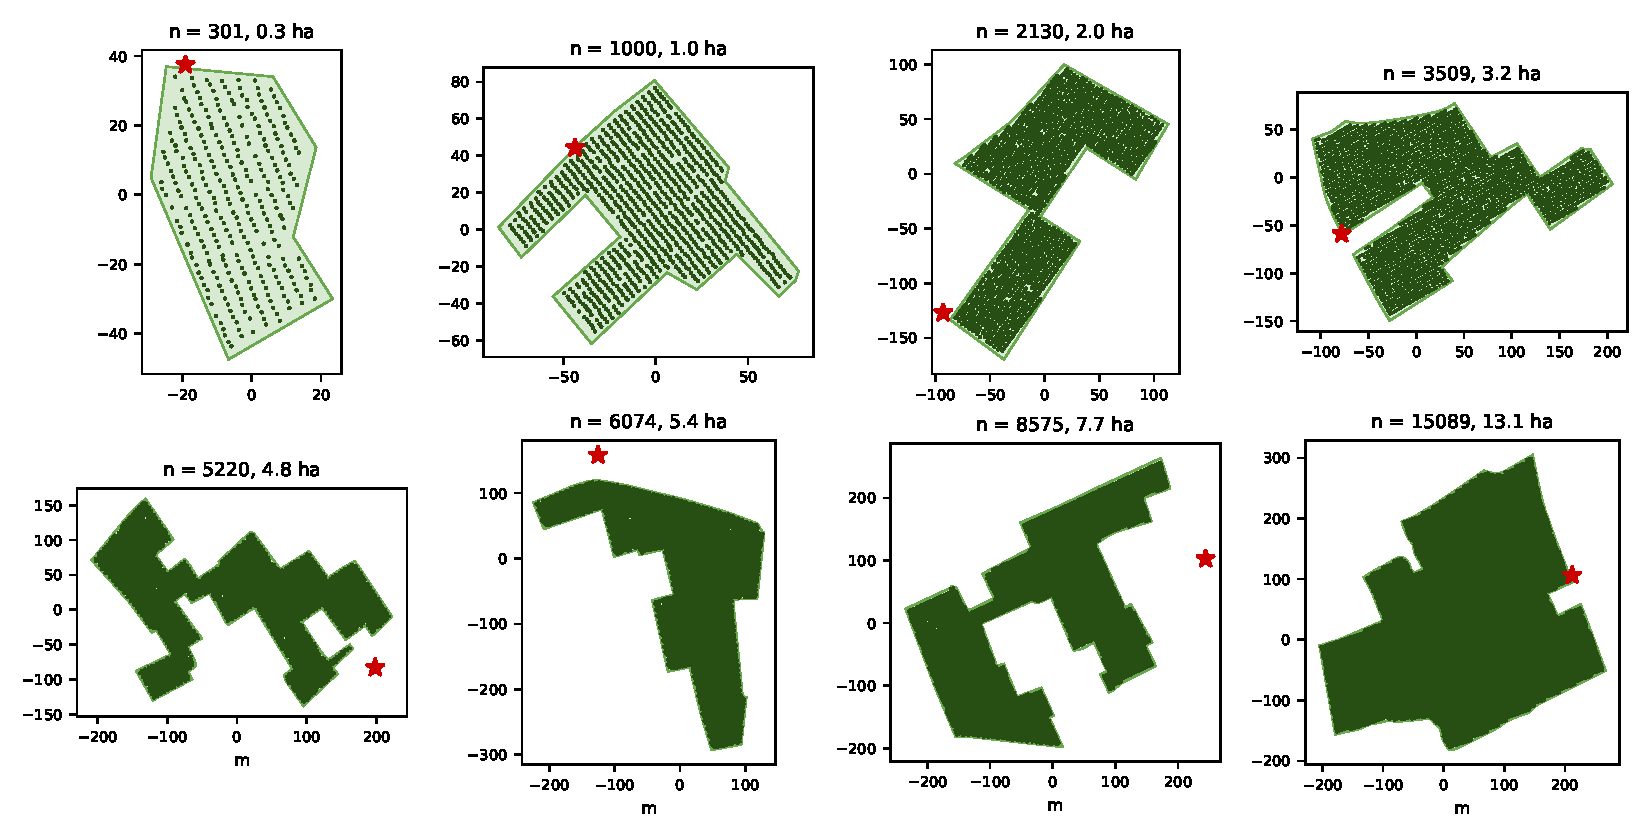
\includegraphics[width=\textwidth]{figs/fig_osm.pdf}
\caption{On altı gerçek bahçe sınırından sekizi (OpenStreetMap,
Isparta), üretilen ağaç kafesi ve depo (yıldız) ile birlikte}\label{fig:osm}
\end{figure}

\subsection{Yöntemler}
\begin{description}
\item[PSB+LNS (bu çalışma).] Algoritma~\ref{alg:psb}; tek atış PSB sonucu ve her
LNS iyileşmesi zaman damgasıyla kaydedilmiştir.
\item[LKH-3.] Sürüm 3.0.13, \texttt{MTSP\_OBJECTIVE = MINMAX}, \texttt{RUNS = 1};
üç yapılandırmada çalıştırılmıştır: \emph{varsayılan}; \emph{ayarlı}, yani iki bahçe
($n=467$ ve $1885$, $k=8$, 120\,s) üzerinde yapılan bir ön denemede sınanan altı ayardan en iyisi olan
\texttt{INITIAL\_TOUR\_}\allowbreak\texttt{ALGORITHM = MTSP} ve
\texttt{MOVE\_TYPE = 2} ($n=1885$ için bu ayar 120\,s'de \num{61249} değerine ulaşmış, varsayılan
ayar ise 600\,s sonunda \num{107222} değerinde kalmıştır); ve \emph{sıcak başlangıçlı}, yani tek atış
PSB çözümünden başlatılan ayarlı yapılandırma (\texttt{INITIAL\_TOUR\_}\allowbreak\texttt{FILE}; PSB
süresi bu yapılandırmanın ölçülen süresine dâhil edilmiştir).
\item[Literatürde öne çıkan min--maks mTSP kodları.] Kodu herkese açık olan dört yöntem
çalıştırılmıştır: HSNR \citep{hehao2022} (C++ kaynak kodu, \texttt{-O3} ile derlenmiş),
MA \citep{hehao2023} ve MILS \citep{hehaoxia2024} (yazarlarca dağıtılan Linux yürütülebilir
dosyaları) ve HGA \citep{mahmoudinazlou2024} (Julia kaynak kodu, tek iş parçacığı);
her biri varsayılan parametreleriyle, tek koşu hâlinde, bütçeye eşit bir duvar saati süre sınırıyla
ve koşuyu erken sonlandıramayan bir durdurma ölçütüyle çalıştırılmıştır. ITSHA \citep{zheng2022} ve
pekiştirmeli öğrenme tabanlı CMSA \citep{rodriguez2026} için açık kod bulunmamaktadır. MA
ve MILS yürütülebilir dosyaları, örnek başlığındaki şehir sayısını depo dâhil olarak
yorumlamaktadır; bu dosyalarla birlikte dağıtılan örnek dosyaları ise sayıyı depo hariç vermekte ve bu durum
son müşterinin uyarı verilmeden atlanmasına yol açmaktadır; bu nedenle başlık $n+1$ ile yazılmış ve her müşterinin
döndürülen rotalarda tam olarak bir kez yer aldığı doğrulanmıştır. MA yaklaşık $1.6\times10^{-7}n^2$\,GB
bellek gerektirdiğinden 15\,089 ağaçlı bahçede çalıştırılmamıştır (tahmini 36\,GB).
\end{description}

\subsection{Protokol ve ölçütler}
Her koşuda tek çekirdek kullanılmıştır. Deneyler, 12 çekirdekli/24 iş parçacıklı bir AMD Ryzen~9 3900X
işlemci ve 46\,GB bellek bulunan bir makinede yürütülmüştür; yöntemler iç içe sıralanarak 20 koşu eşzamanlı
çalıştırılmış, böylece makine yükünün tüm yöntemleri eşit biçimde etkilemesi sağlanmıştır. Zaman bütçesi
$n<1000$ için 120\,s, $n<5000$ için 300\,s, diğer durumlarda 600\,s olarak belirlenmiştir. PSB+LNS ve LKH-3
\SeedsMain{} tohumla (LNS ve LKH-3 için rastgele tohum; tek atış PSB sonucu
deterministiktir), literatürde öne çıkan dört kod ise tek tohumla çalıştırılmıştır. İyileşme izleri,
çıktı satırları üretildikçe duvar saatine göre zaman damgasıyla kaydedilmiştir; bir $b$ bütçesi,
$1.02\,b$ anına kadar ($b\ge 60$\,s için artı 2\,s) bir çözüm raporlanmışsa karşılanmış
sayılmış ve her yöntemin nihai sonucu, ilgili sınıf bütçesinin bu tolerans içinde kalan en iyi
çözümü olarak alınmıştır.

Her örnek ve $k$ değeri için \emph{best} (en iyi), herhangi bir yöntem, tohum ve süreyle bulunan en küçük
tamamlanma süresidir. Raporlanan ölçüler şunlardır: $t\in\{0.1,1,10,60\}$\,s bütçelerinde
ve bütçe sonunda $C_{\max}(t)/\text{best}-1$ sapması (çözüm yoksa ``çözüm yok''),
PSB+LNS'nin bir rakipten kesin olarak daha iyi olduğu örneklerin payı
(tohum ortalamaları kullanılarak) ve örnek başına ortalama nihai sapmalara
örnekler genelinde uygulanan çift yönlü Wilcoxon işaretli sıra testidir. Aynı temel
nokta kümesinin farklı $k$ değerleri bağımsız örnekler olmadığından $p$-değerleri
doğrulayıcı değil, keşifsel karşılaştırma ölçütleri olarak yorumlanmıştır.
